 \documentclass[11pt, oneside]{article}   	% use "amsart" instead of "article" for AMSLaTeX format
\usepackage{geometry}                		% See geometry.pdf to learn the layout options. There are lots.
\geometry{letterpaper}                   		% ... or a4paper or a5paper or ... 
%\geometry{landscape}                		% Activate for for rotated page geometry
%\usepackage[parfill]{parskip}    		% Activate to begin paragraphs with an empty line rather than an indent
\usepackage{graphicx}				% Use pdf, png, jpg, or eps§ with pdflatex; use eps in DVI mode
								% TeX will automatically convert eps --> pdf in pdflatex		
\usepackage{amssymb}
\usepackage{amsmath}
\usepackage{parskip}
\usepackage{color}
\usepackage{hyperref}

\title{Derivative formula}
%\author{The Author}
%\section{}
%\subsection*{}
\date{}							% Activate to display a given date or no date

\graphicspath{{/Users/telliott_admin/Dropbox/Tex/png/}}
% \begin{center} 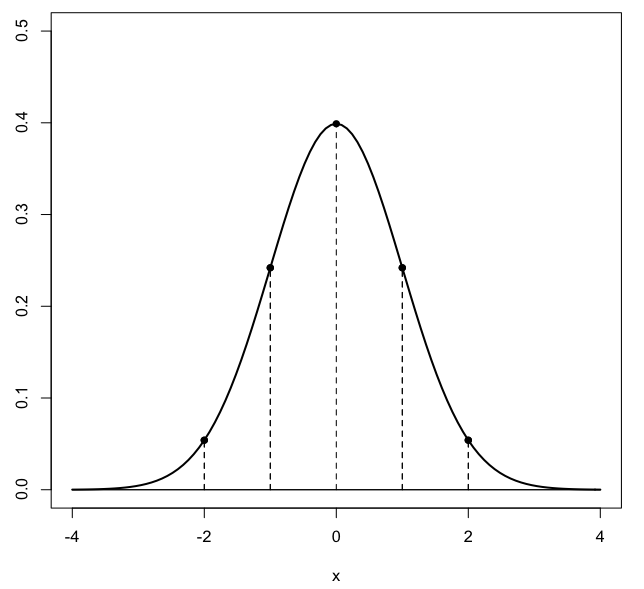
\includegraphics [scale=0.4] {gauss3.png} \end{center}
\begin{document}
\maketitle
\Large

Kaplan gives some rules for computing residues, which we explore in this chapter.

\textbf{RULE I}  At a simple pole $z_0$ (that is, a pole of first order),
\[ \text{Res } [f(z),z_0] = \lim_{z \rightarrow z_0} (z-z_0) f(z) \]

\subsection*{example}
The example is one we already worked.
\[ f(z) = \frac{1}{z^2 + 1} = \frac{1}{(z - i)(z + i)} \]
\[ \text{Res } [f(z),z=i] = \lim_{z \rightarrow i} (z-i) \frac{1}{(z - i)(z + i)} \]
\[ = \lim_{z \rightarrow i} \frac{1}{z + i} = \frac{1}{2i} \]

\subsection*{review}

To summarize the key points about Cauchy 2 and residues, this is the theorem
\[ \oint_C \frac{f(z)}{z - z_0} \ dz = 2 \pi i \ f(z_0) \]
By definition the residue at a simple pole is defined to be
\[ b_1 = \lim_{z \rightarrow z_0} (z-z_0) \ f(z)  \]
Just think of it as in the limit that $z \rightarrow z_0$, the denominator $z-z_0$ on the left is a constant, so we can multiply both sides by $z - z_0$ to obtain the result for the residue.
\[ \oint f(z) \ dz = 2 \pi i \ \sum \text{ Res } \]
The value of the integral is $2 \pi i$ times the sum of all the residues enclosed by the path.

\subsection*{derivative rule}

We show here that
\[ f'(a) = \frac{1}{2 \pi i} \ \oint_C \frac{f(z)}{(z-a)^2} \ dz \]
and there are more formulas for higher derivatives.
Therefore
\[ 2 \pi i \ f'(a) =  \oint_C \frac{f(z)}{(z-a)^2} \ dz \]

Again, the Cauchy formula is:
\[ \oint_C \frac{f(z)}{z-z_0} \ dz = 2 \pi i f(z_0) \]
rewrite with $a$ for $z_0$
\[ \oint_C \frac{f(z)}{z-a} \ dz = 2 \pi i f(a) \]

We take the partial with respect to $a$ of both sides:
\[ \frac{\partial}{\partial a} ( \frac{f(z)}{z-a} ) = \frac{f(z)}{(z-a)^2} \]
so
\[ \oint_C \frac{f(z)}{(z-a)^2} \ dz = 2 \pi i f'(a) \]
Thus
\[ f'(a) = \frac{1}{2 \pi i} \ \oint_C \frac{f(z)}{(z-a)^2} \ dz \]
More generally
\[ f^n(a) = \frac{n!}{2 \pi i} \ \oint_C \frac{f(z)}{(z-a)^{n+1}} \ dz \]
So
\[ \frac{2 \pi i}{n!} f^n(a) = \oint_C \frac{f(z)}{(z-a)^{n+1}} \ dz \]

\subsection*{example}
\[ \oint_C \frac{e^z}{z^3 - z^2 - 5z - 3} = \oint_C \frac{e^z}{(z+1)^2 (z-3)} \]

Recall the general formula
\[ f'(a) = \frac{1}{2 \pi i} \ \oint_C \frac{f(z)}{(z-a)^2} \ dz \]

If the contour includes $z = -1$ but not $z = 3$ then
\[ f(z) = \frac{e^z}{(z-3)} \]
so
\[ f'(z) = \frac{(z-4)e^z}{(z-3)^2} \]

Hence
\[ \oint_C \frac{e^z}{z^3 - z^2 - 5z - 3} \ dz = \oint_C \frac{e^z}{(z+1)^2 (z-3)} \]
\[ = \oint_C \frac{f(z)}{(z+1)^2} \ dz \]
for $f(z) = e^z/(z-3) $ and
\[ = 2 \pi i f'(-1) = 2 \pi i \ \frac{-5}{e} \ \frac{1}{(-4)^2} \]
\[ = \frac{-5 \pi i}{8 e}  \]

\subsection*{Kaplan}
Here is rule II from Kaplan.  Rule I is in the previous section.

\textbf{RULE II}  At a pole of order $N$ ($N = 2, 3, \dots$),
\[ \text{Res } [f(z),z_0] = \lim_{z \rightarrow z_0} (z-z_0) \frac{g^{(N-1)}(z)}{(N-1)!} \]
where 
\[ g(z) = (z-z_0)^N f(z) \]

\subsection*{example}
\[ f(z) = \frac{1}{z(z-2)^2} \]
We have a pole of first order at $z_0=0$ and one of second order at $z_0=2$.  At the first
\[ \text{Res }(0) = \lim_{z \rightarrow 0} \frac{1}{(z-2)^2} = \frac{1}{4} \]

For the other one, remove the factor of $1/(z-2)^2$ and compute the $N-1$ (first) derivative of what's left
\[ \frac{d}{dz} \frac{1}{z} =  - \frac{1}{z^2} \]
\[ \text{Res } (2) = \lim_{z \rightarrow 2} -\frac{1}{z^2} = -\frac{1}{4} \]
Don't forget to divide by $(N-1)!$, which is just $1$ in this case.  The total is just zero.

As a check, let's do this by partial fractions.
\[ \frac{1}{z(z-2)^2} = \frac{A}{(z-2)^2} +  \frac{B}{z(z-2)} +  \frac{C}{z}  \]
Hence in putting all terms over a common denominator, for the numerator we have
\[ 1 = Az + B(z-2) + C(z-2)^2 \]
From which we get three equations:
\[ -2B + 4C = 1 \]
\[ Az + Bz - 4Cz = 0 \]
\[ Cz^2 = 0 \]
Hence $C = 0$, so $B = -1/2$ and $A = 1/2$ and we obtain
\[ \frac{1}{z(z-2)^2} = \frac{1/2}{(z-2)^2} - \frac{1/2}{z(z-2)} \]
which we check by doing
\[ 1/2 \cdot z - 1/2 \cdot (z-2) = 1 \]
So how to deal with 
\[ \frac{1/2}{(z-2)^2} - \frac{1/2}{z(z-2)} \]
The first term has a pole of order $2$ at $z_0 = 2$.  We remove that factor and compute the $N-1$ (first) derivative of what's left, which is just zero.  

For the second term, we have two simple poles at $z_0=0$ and $z_0=2$.  The residues are
\[ \text{Res } (0) = \lim_{z \rightarrow 0} z \cdot \frac{1}{z(z-2)} = - \frac{1}{2} \]
\[ \text{Res } (2) = \lim_{z \rightarrow 2} (z-2) \cdot \frac{1}{z(z-2)} = \frac{1}{2} \]
which adds up to zero.

\subsection*{example}
\[ f(z) = \frac{1}{z^4 + z^3 - 2z^2} \]
where $C$ is the circle $|z| = 3$ with positive orientation.

The denominator can be factored as
\[ z^2(z^2 + z - 2) = z^2(z + 2)(z - 1) \]
so
\[ f(z) = \frac{1}{z^2(z + 2)(z - 1)} \]
There is a pole of order 2 at the origin and simple poles at 1 and -2.  All of these lie within the contour $|z| = 3$.
\[ \text{Res }(1) = \lim_{z \rightarrow 1} (z-1) \ f(z) = \lim_{z \rightarrow 1} \frac{1}{z^2 (z + 2)} = \frac{1}{3} \]
\[ \text{Res }(-2) = \lim_{z \rightarrow -2} (z+2) \ f(z) = \lim_{z \rightarrow -2} \frac{1}{z^2 (z - 1)} = -\frac{1}{12} \]
For the double pole, we remove the factor of $1/z^2$, take the first derivative of what's left
\[ \frac{d}{dz} \ \frac{1}{z^2 + z - 2} = \frac{(-1)(2z + 1)}{(z^2 + z - 2)^2} \]
Evaluate at zero and obtain.
\[ \text{Res }(0) = - \frac{1}{4} \]
The total of the residues is
\[ \frac{1}{3} -\frac{1}{12} - \frac{1}{4} = 0 \]
As Mathews and Howell say:
\begin{quote}The value 0 for the integral is not an obvious answer, and all of the preceding calculations are required to find it.\end{quote}

\subsection*{example}
\[ f(z) = \frac{1 + e^z}{z^2} + \frac{2}{z} \]
We can break this up into its two component parts.  For the first term, the pole is of order $m = 2$ at $z_0 = 0$.  We remove the $z^2$ term and take the $m-1 = 1$ derivative
\[ (1 + e^z)' = e^z \]
Remember to divide by $(m-1)!$, leaving $e^z$ which is evaluated at the pole giving a residue
\[ \text{Res }(0) = e^0 = 1 \]

The other term is just $2$ times the standard
\[ \oint \frac{1}{z} \ dz = 2 \pi i \]
Here $I = 4 \pi i$ and the residue is $2$.  Alternatively just use
\[ I = 2 \pi i f(z_0) = 4 \pi i \]
where $f = 2$.

The total of the residues is $3$ and the value of the integral is $6 \pi i$.



\subsection*{example}
\[ f(z) = \frac{e^z}{z(z-1)^2} \]
We have a pole of first order at $z=0$ and one of second order at $z=1$.  At the first
\[ \text{Res } [f(z),z=0] = \lim_{z \rightarrow 0} \frac{e^z}{(z-1)^2} = 1 \]

For the other one, remove the factor of $1/(z-1)^2$ and compute the $N-1$ (first) derivative of what's left
\[ \text{Res } [f(z),z=1] = \lim_{z \rightarrow 1} \ [ \ \frac{e^z}{z} \ ]' \ \]
\[ = \frac{e^z z - e^z}{z^2} \ \bigg |_1 =  0 \]
Hence
\[ \oint f(z) \ dz = 2 \pi i \ [ \ \sum  \text{Res } \ ] \ = 2 \pi i \]

\subsection*{example}
\[ f(z) = \frac{1}{z(z-2)^4} \]
We have a pole of first order at $z=0$ and one of fourth order at $z=2$.  At the first
\[ \text{Res } [f(z),z=0] = \lim_{z \rightarrow 0}  z \ \frac{1}{z(z-2)^4} \]
\[ =  \lim_{z \rightarrow 0} \ \frac{1}{(z-2)^4}  = \frac{1}{(-2)^4} =  \frac{1}{16} \]

For the other pole recall that
\[ \frac{2 \pi i}{n!} f^n(a) = \oint_C \frac{f(z)}{(z-a)^{n+1}} \ dz \]

We remove the factor of $1/(z-2)^4$ leaving $f(z) = 1/z$ and then compute the $N-1$ (third) derivative of what's left
\[ \text{Res } [f(z),z=2] = \frac{1}{n!} \ \lim_{z \rightarrow 2} \ [ \ \frac{1}{z} \ ]''' \ \]
\[ f(z) = z^{-1} \]
\[ f'(z) = - z^{-2} \]
\[ f''(z) = 2 z^{-3} \]
\[ f'''(z) = -6 z^{-4} \]
\[  \lim_{z \rightarrow 2} \ [ \ \frac{1}{z} \ ]''' = - \frac{6}{16} \]
Don't forget to divide by $(N-1)!$, which is $3! = 6$ in this case.  That leaves
\[ \text{Res } [f(z),z=2] = - \frac{1}{16} \]

The total of the residues is just zero.  

This problem is from Brown and Churchill (p. 234), which they work by doing Laurent series.  They get a different answer, namely $-\pi i/8$.  

The reason is that they integrate over the contour $0 < | z - 2 | < 2$, which includes the second pole, but not the first.  Multiplying by $2 \pi i$ gives their result.

\end{document}  
